% !TeX spellcheck = fr_FR
\chapter{Chapitre 9 : Frontend}

\section*{Panorama}

Ce chapitre présente l'architecture du \textbf{frontend} et l'ergonomie de l'application. Il se lit comme un guide de visite: la carte interactive (page d'accueil), l'outil d'identification des problèmes, la gestion des données persistantes, et la génération de rapports. Pour les aspects API et modèles de données, voir \textbf{Chapitre 8}. Ici nous décrivons le cycle de vie des requêtes, les seuils de zoom, le rendu des marqueurs et la logique des info-bulles.

\medskip
\noindent
\begin{figure}[h]
  \centering
  \includegraphics[width=0.95\textwidth]{../figures/chap9/main_page.png}
  \caption[Page d'accueil]{Vue générale de la page d'accueil}
  \label{fig:frontend-index-main}
\end{figure}

\begin{figure}[h]
  \centering
  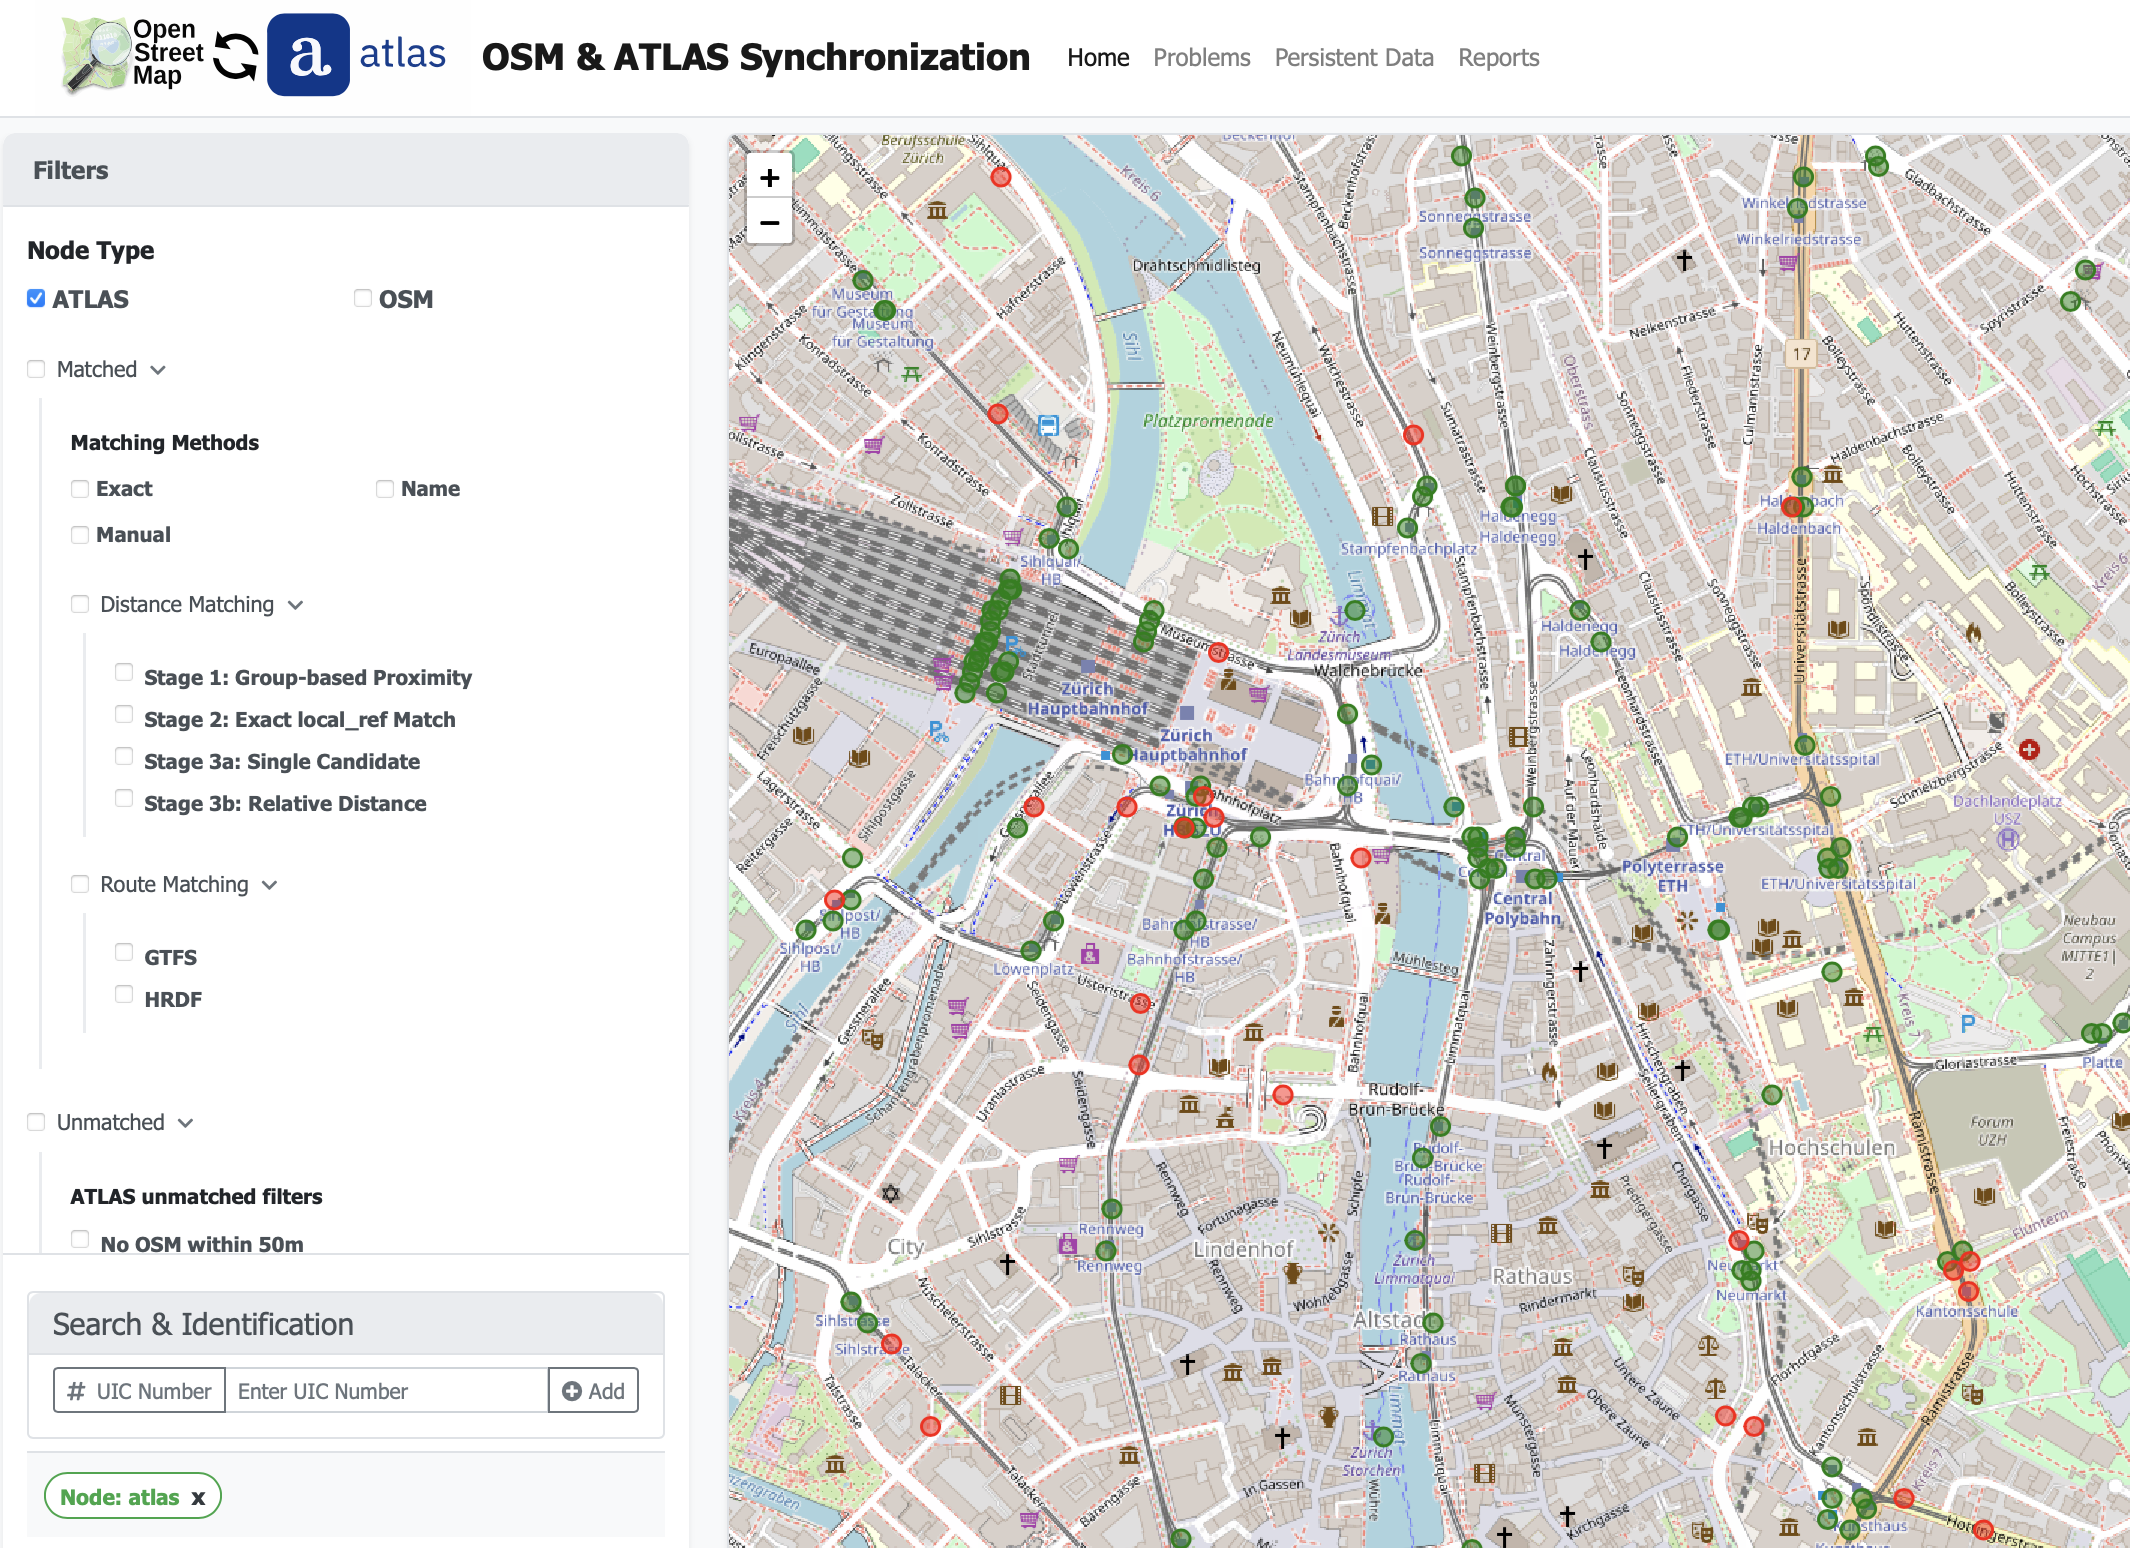
\includegraphics[width=0.95\textwidth]{../figures/chap9/atlas filter activ main page.png}
  \caption[Filtre ATLAS (Zurich)]{Filtre ATLAS activé — ville de Zurich}
  \label{fig:frontend-index-filters}
\end{figure}

\section{Pages et navigation}

L'application comporte quatre vues principales :
\begin{itemize}
  \item \textbf{Carte (Index)} — exploration des arrêts, filtres riches, info-bulles, et un \emph{Top~N} des plus grandes distances. (Template: \texttt{templates/pages/index.html})
  \item \textbf{Problèmes} — tri, filtrage et résolution guidée des anomalies avec contexte cartographique local. (\texttt{templates/pages/problems.html})
  \item \textbf{Données persistantes} — revue et gestion des solutions/notes persistées entre imports. (\texttt{templates/pages/persistent\_data.html})
  \item \textbf{Rapports} — page dédiée de configuration et rendu PDF/CSV via backend (\texttt{templates/pages/reports.html}, cf. \S\ref{subsec:rapports}).
\end{itemize}

Chaque page est construite en HTML Jinja\citeref{ref:jinja_docs}, stylisée par les feuilles CSS du dossier \texttt{static/css}, et animée par du JavaScript modulaire dans \texttt{static/js}.

\section{Carte interactive (Index)}

\subsection{Cycle de vie des requêtes}
La carte (Leaflet\citeref{ref:leaflet_docs}) initialise une vue par défaut et \textbf{anti-rebondit} les événements \texttt{moveend}/\texttt{zoomend} (\(\sim\)320~ms) avant de charger la nouvelle fenêtre d'affichage. Les requêtes en vol sont \textbf{annulées} lorsque l'utilisateur se déplace à nouveau, ce qui évite les rendus obsolètes. Les paramètres envoyés à l'API incluent la \textit{bbox} et les filtres actifs. Références côté serveur: \texttt{/api/data} and \texttt{/api/stop\_popup} (voir Chap.~8 pour la logique et la sérialisation).

\begin{itemize}
  \item \textbf{Seuils de zoom} — pas de marqueurs en dessous de \(z<13\); les \textit{polylignes} de liaison ne s'affichent qu'à partir de \(z\ge 14\).
  \item \textbf{Petits ensembles à faible zoom} — une \textit{sonde} plafonnée à \(\leq 250\) entrées permet d'afficher un petit ensemble même à bas zoom; sinon, une bannière invite à zoomer.
  \item \textbf{Milieu de zoom} — résultats plafonnés (\(\leq 500\)).
  \item \textbf{Fort zoom} — plafond levé: \emph{tous} les marqueurs de la fenêtre sont renvoyés.
\end{itemize}

\noindent
\textit{Capture d'écran} : bannière ``zoomez'' et apparitions des marqueurs.

\begin{figure}[h]
  \centering
  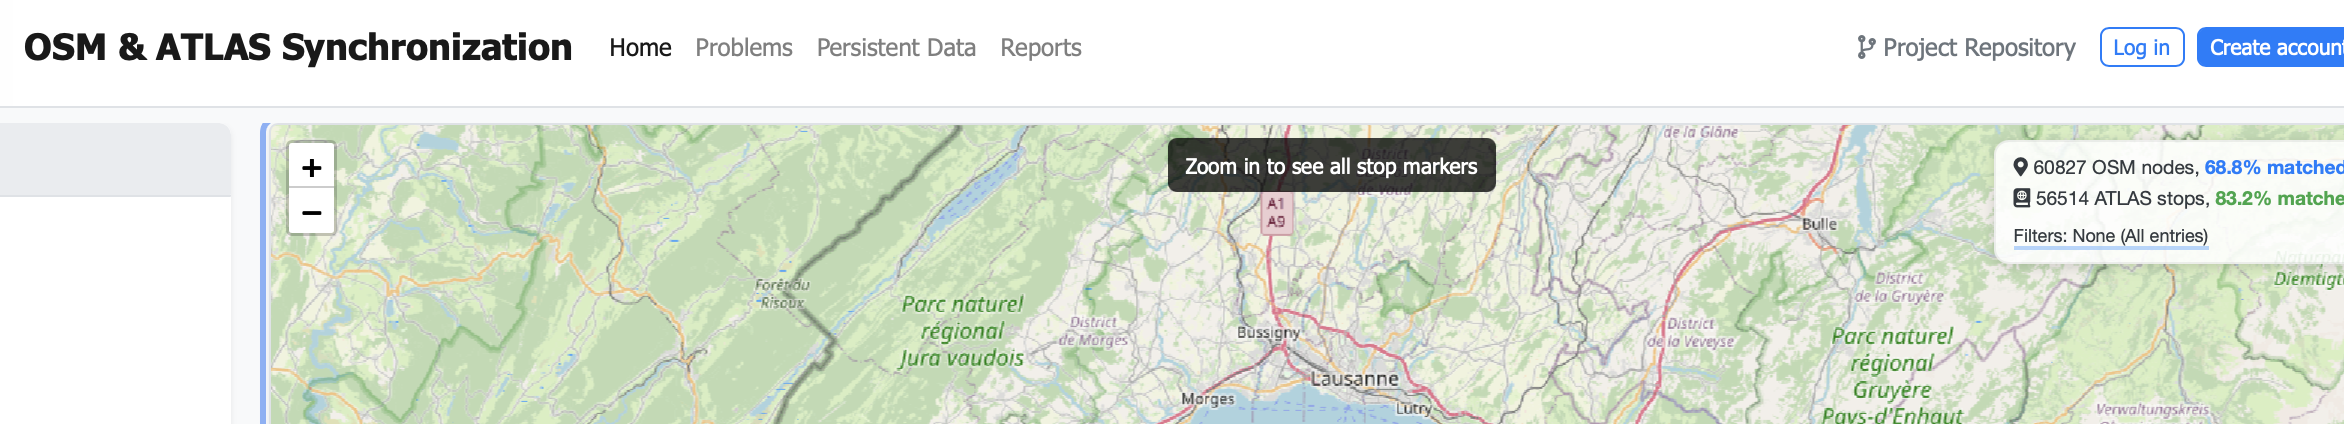
\includegraphics[width=0.9\textwidth]{../figures/chap9/zoom_in_to_see_all_stop_markers.png}
  \caption[Bannière de zoom]{Bannière politique de rendu selon le niveau de zoom}
  \label{fig:frontend-zoom-banner}
\end{figure}

\subsection{Rendu des marqueurs et des lignes}
Le rendu privilégie des cercles Canvas/SVG légers jusqu'au zoom \(z<18\). Au-delà, certaines icônes \textit{lettrees} (\texttt{D}, \texttt{P}, \texttt{S}) sont utilisées pour signaler \textit{duplicate}, \textit{platform}, \textit{station}. Les icônes DOM identiques sont \textbf{mises en cache} pour éviter les reconstructions inutiles.

Lorsque des marqueurs se superposent exactement, un \textbf{décalage circulaire} subtil est appliqué pour éviter l'occlusion. Les ajouts au calque sont \textbf{lotis} (\(\sim\)150–200 par lot) afin de préserver la réactivité du thread principal.

Les paires appariées (ATLAS–OSM) peuvent afficher une \textbf{ligne de liaison} (verte par défaut; violette pour un match manuel, en pointillés si non persistant) lorsque les deux extrémités sont visibles et que le zoom le permet.

% (figure déplacée vers la section Filtres)

\subsection{Info-bulles et chargement paresseux}
Le contenu des popups est rendu par un \textbf{moteur de gabarits côté client} (\texttt{PopupRenderer}). Un premier clic déclenche un appel à \texttt{/api/stop\_popup} qui renvoie des détails enrichis (noms, opérateurs, routes, notes). Les vues \textit{unifiées} permettent d'inspecter \textbf{toutes les correspondances} d'un nœud (ATLAS \emph{vs} OSM) sans recharger la page. Les popups sont déplaçables et conservent une \textit{ligne d'ancrage} lors des déplacements/zooms.

Pour les entrées non appariées, un bouton \texttt{Match to} apparaît dans l'info-bulle. La sélection d'une cible opposée (ATLAS \(\leftrightarrow\) OSM) déclenche la création d'un match manuel via \texttt{/api/manual\_match}. Cette action est cohérente avec le \textit{workflow} décrit au Chap.~8 (persistance optionnelle).

\begin{figure}[h]
  \centering
  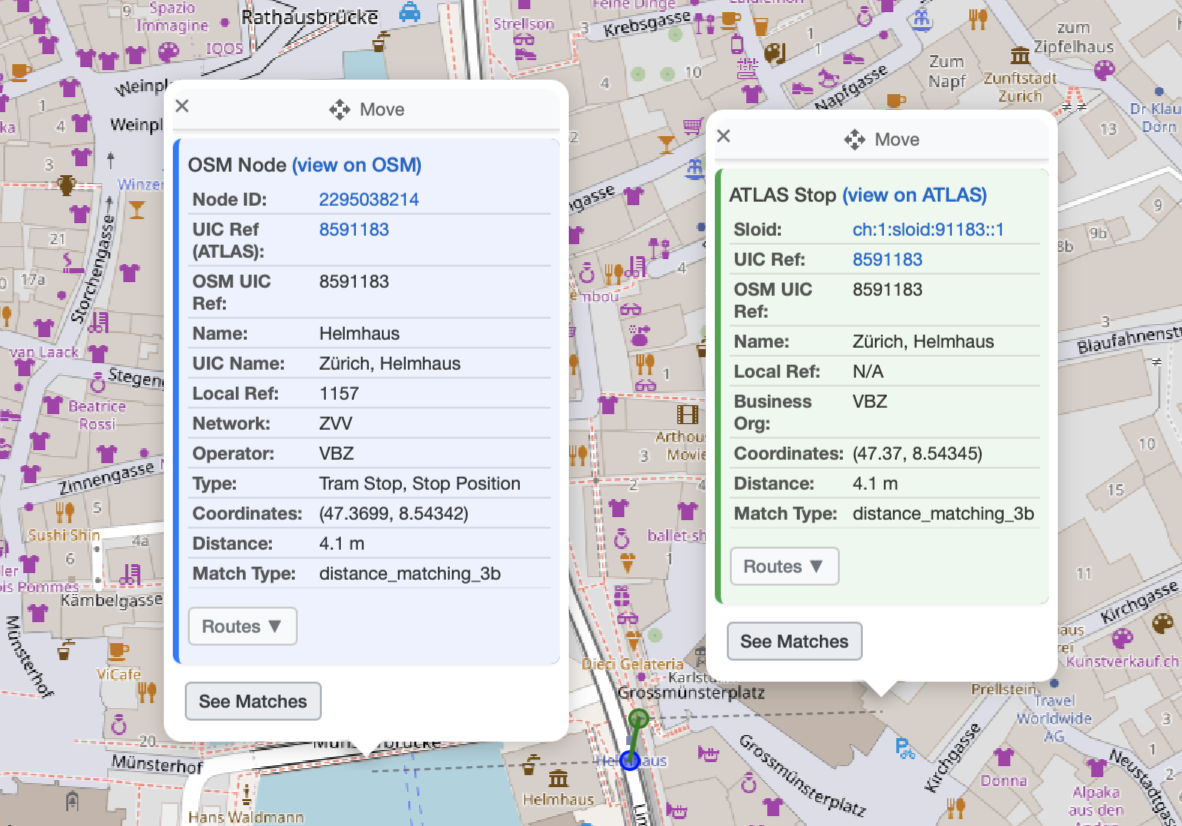
\includegraphics[width=0.85\textwidth]{../figures/chap9/popups.png}
  \caption[Info-bulles]{Info-bulles}
  \label{fig:frontend-popups}
\end{figure}

\subsection{Panneau de filtres et recherche}
Le panneau de gauche agrège des filtres \textbf{par domaines fonctionnels} :
\begin{itemize}
  \item \textbf{Type de nœud} (ATLAS/OSM) et \textbf{Type d'arrêt} (\textit{Matched}, \textit{Unmatched}, \textit{Station}).
  \item \textbf{Méthodes d'appariement}: Exact, Name, Manual; \textbf{Distance Matching} (stages 1, 2, 3a, 3b); \textbf{Route Matching} (GTFS, HRDF).
  \item \textbf{Top N Distances} — surcouche légère pour inspecter rapidement les plus grandes distances.
  \item \textbf{Transports} (station, platform, stop\_position, ferry, aerialway, tram, etc.).
  \item \textbf{Opérateurs ATLAS} — \textit{dropdown} dédié avec recherche (chargé depuis \texttt{/api/operators}).
  \item \textbf{Filtres spéciaux} — afficher uniquement les \textit{duplicates} ATLAS.
\end{itemize}

La zone \textit{Active Filters} affiche des \textbf{"chips"} cliquables (ET/OU) pour retirer rapidement un critère. Un \textbf{sélecteur de type de recherche} (numéro UIC, SLOID ATLAS, OSM Node ID, Route ID) ajuste dynamiquement le champ de saisie et les actions associées. Un \textbf{résumé d'en-tête} interroge \texttt{/api/global\_stats} pour afficher des indicateurs utiles (ex.: pourcentage de nœuds appariés) synchronisés avec les filtres.

\begin{figure}[h]
  \centering
  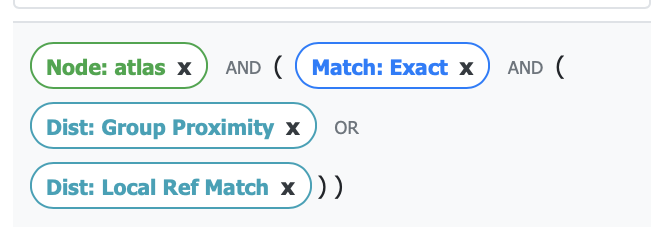
\includegraphics[width=\textwidth]{../figures/chap9/filter_chips_index.png}
  \caption[Filtres — chips actifs]{Panneau de filtres avec \og chips \fg{} actifs}
  \label{fig:frontend-filters-chips}
\end{figure}

\begin{figure}[h]
  \centering
  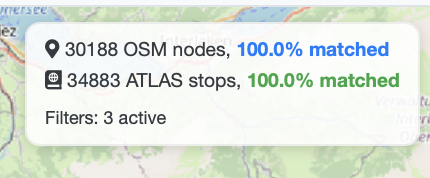
\includegraphics[width=\textwidth]{../figures/chap9/stats box.png}
  \caption[Résumé d'en-tête]{Résumé d'en-tête avec statistiques globales. 3 filtres actifs}
  \label{fig:frontend-filters}
\end{figure}

\section{Outil Problèmes}

La page \textbf{Problèmes} combine : un panneau de filtres repliable (type d'anomalie, tri, opérateurs, priorité), une \textbf{carte de contexte} locale (\(\pm 0.02^\circ\)), et un \textbf{panneau de résolution} avec navigation par entrées. Les raccourcis clavier accélèrent la revue (\(\rightarrow\)/Espace: suivant, \(\leftarrow\): précédent, \(\uparrow\)/\(\downarrow\): défilement).

Les boutons d'action proposent des solutions pré-remplies (selon le type d'anomalie), la \textbf{persistance} des corrections, et l'édition de \textbf{notes} ATLAS/OSM. Le \textit{toggle} \texttt{Auto-Persist} permet de rendre persistantes toutes les nouvelles solutions/notes ; l'information est stockée pour être \textbf{réappliquée automatiquement} lors d'un prochain import (voir \S\,\emph{Persistance} et Chap.~8).

\begin{figure}[h]
  \centering
  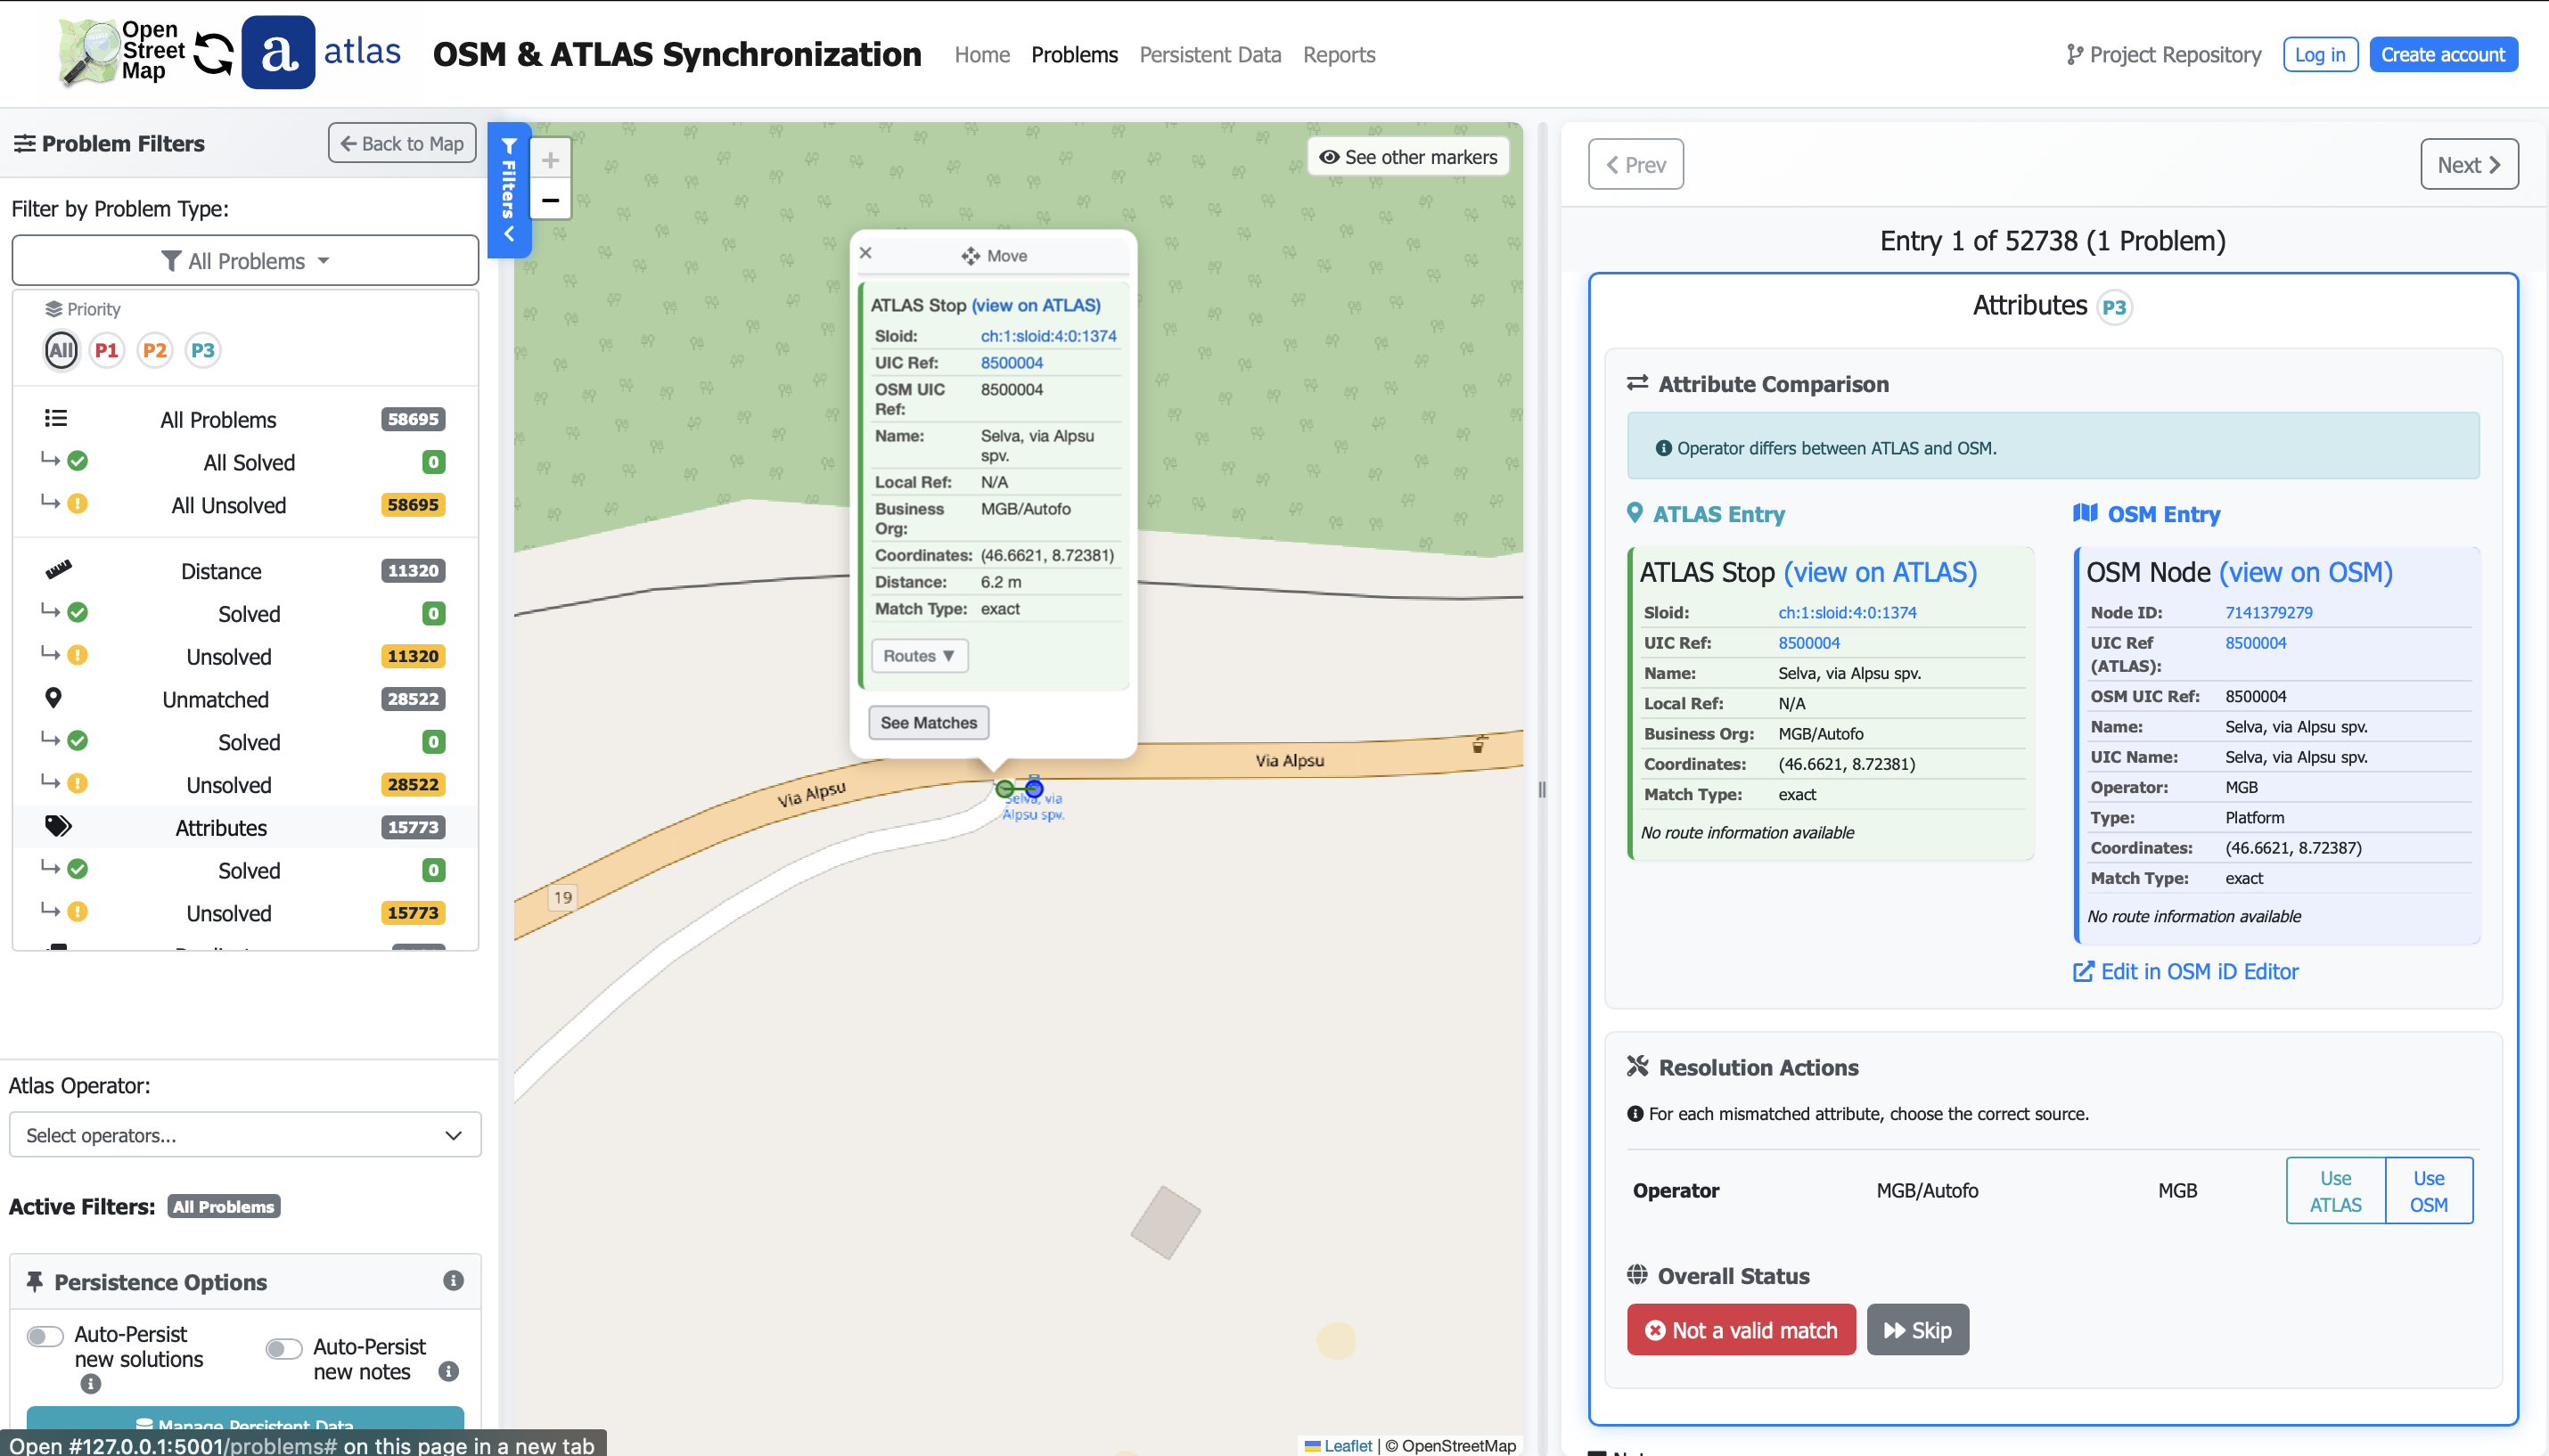
\includegraphics[width=0.9\textwidth]{../figures/chap9/problems page.png}
  \caption[Page Problèmes — vue d'ensemble]{Page Problèmes — vue d'ensemble : filtres, carte de contexte et panneau de résolution}
  \label{fig:frontend-problems}
\end{figure}

\begin{figure}[h]
  \centering
  \begin{minipage}[b]{0.48\textwidth}
    \centering
    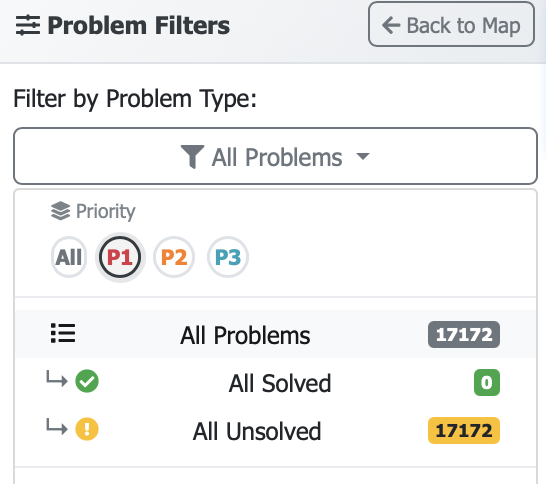
\includegraphics[width=\textwidth]{../figures/chap9/problems priority filter.png}
    \caption*{Filtre de priorité et tri.}
  \end{minipage}\hfill
  \begin{minipage}[b]{0.48\textwidth}
    \centering
    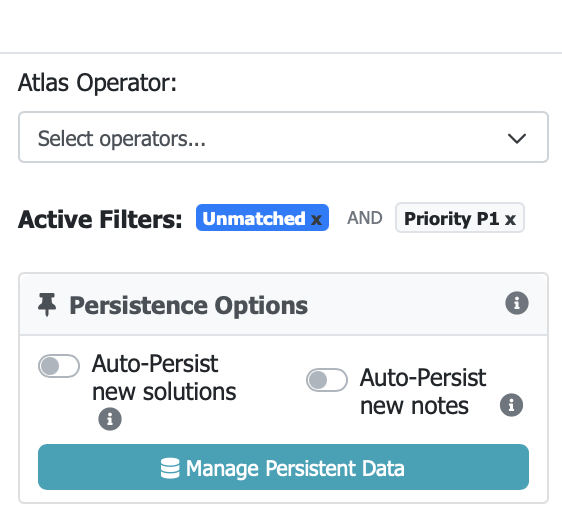
\includegraphics[width=\textwidth]{../figures/chap9/problems fiterchips and persistence options toggles.png}
    \caption*{Chips actifs et options de persistance.}
  \end{minipage}
  \caption[Contrôles — Page Problèmes]{Contrôles de filtrage et options de persistance — Page Problèmes}
\end{figure}

\begin{figure}[h]
  \centering
  \begin{minipage}[b]{0.48\textwidth}
    \centering
    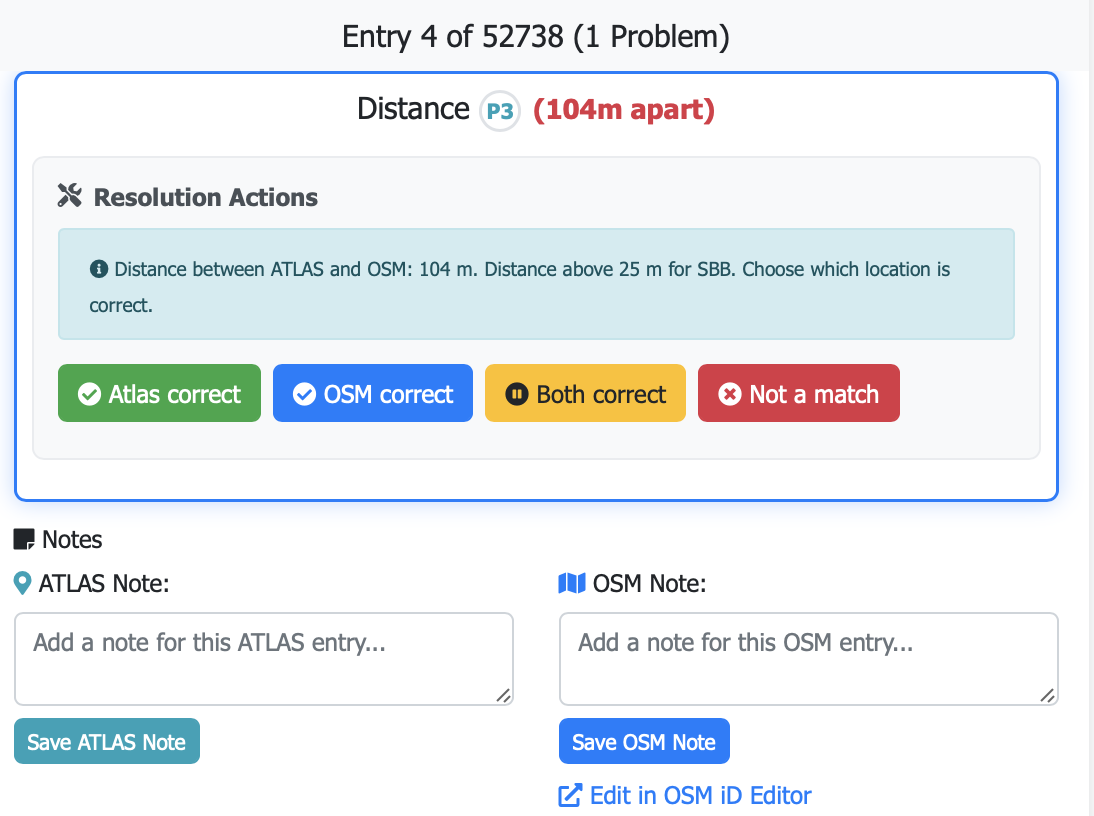
\includegraphics[width=\textwidth]{../figures/chap9/distance problem resolution actions.png}
    \caption*{Actions proposées : problèmes de distance.}
  \end{minipage}\hfill
  \begin{minipage}[b]{0.48\textwidth}
    \centering
    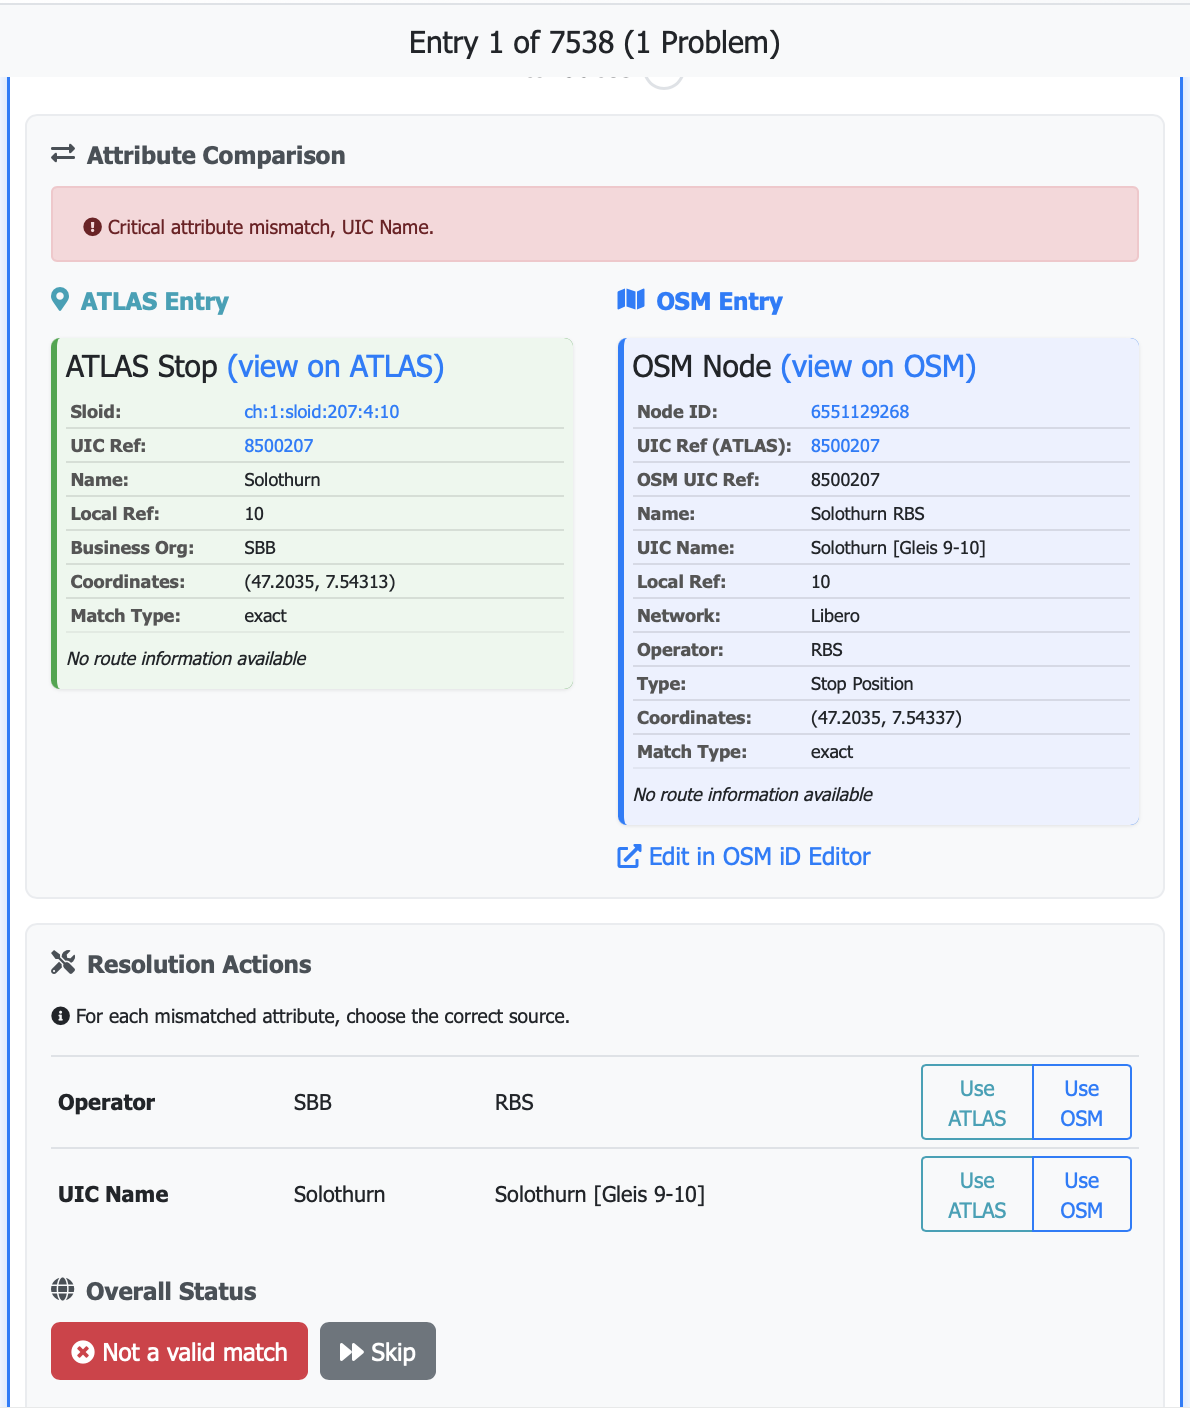
\includegraphics[width=\textwidth]{../figures/chap9/problem resolution actions attributes problem.png}
    \caption*{Actions proposées : problèmes d'attributs.}
  \end{minipage}
  \caption[Panneau de résolution]{Panneau de résolution — actions contextuelles selon le type d'anomalie}
\end{figure}

\section{Données persistantes}

La page \textbf{Données persistantes} distingue les \textit{persistantes} (appliquées après import) des \textit{non persistantes}. On peut filtrer par type (distance, unmatched, attributes, notes) et effectuer des actions massives (\textit{Make All Persistent}, suppression/vidage). Côté serveur, ces opérations appellent les endpoints dédiés décrits au Chap.~8.

\begin{figure}[h]
  \centering
  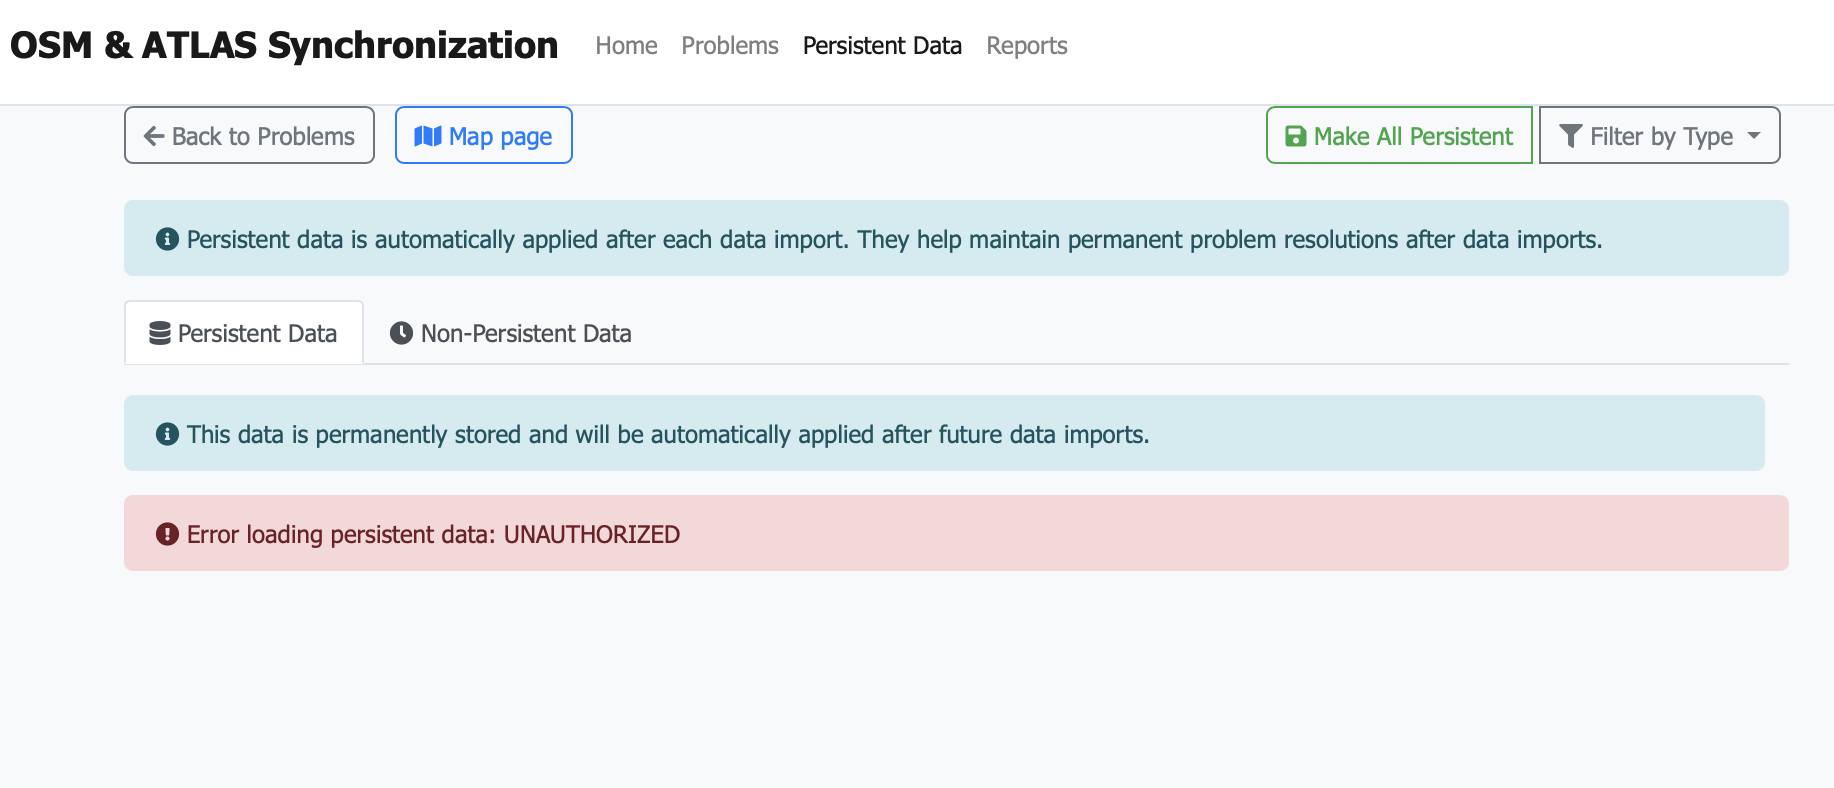
\includegraphics[width=0.9\textwidth]{../figures/chap9/non admin persisten data page.png}
  \caption[Données persistantes (non admin)]{Données persistantes — pour utilisateurs non administrateurs}
  \label{fig:frontend-persistent}
\end{figure}

\section{Rapports et instantanés}
\label{subsec:rapports}

Une \textbf{page dédiée} (\texttt{/reports}) propose un formulaire de configuration pour générer des rapports (\textit{Top Matches}, \textit{Exact}, \textit{Name}, \textit{Duplicates}) en PDF ou CSV via l'endpoint \texttt{/api/generate\_report} (voir Chap.~8). Un \textbf{plafond de 20 téléchargements par IP et par jour} est appliqué côté serveur (limiteur global avec règle spécifique à l'endpoint) pour garantir un usage équitable. Un \textbf{instantané de carte} (\texttt{map\_snapshot.html}) peut afficher un groupe UIC/Opérateur avec marqueurs et liaisons, utile pour des annexes ou l'intégration dans le mémoire.

\begin{figure}[h]
  \centering
  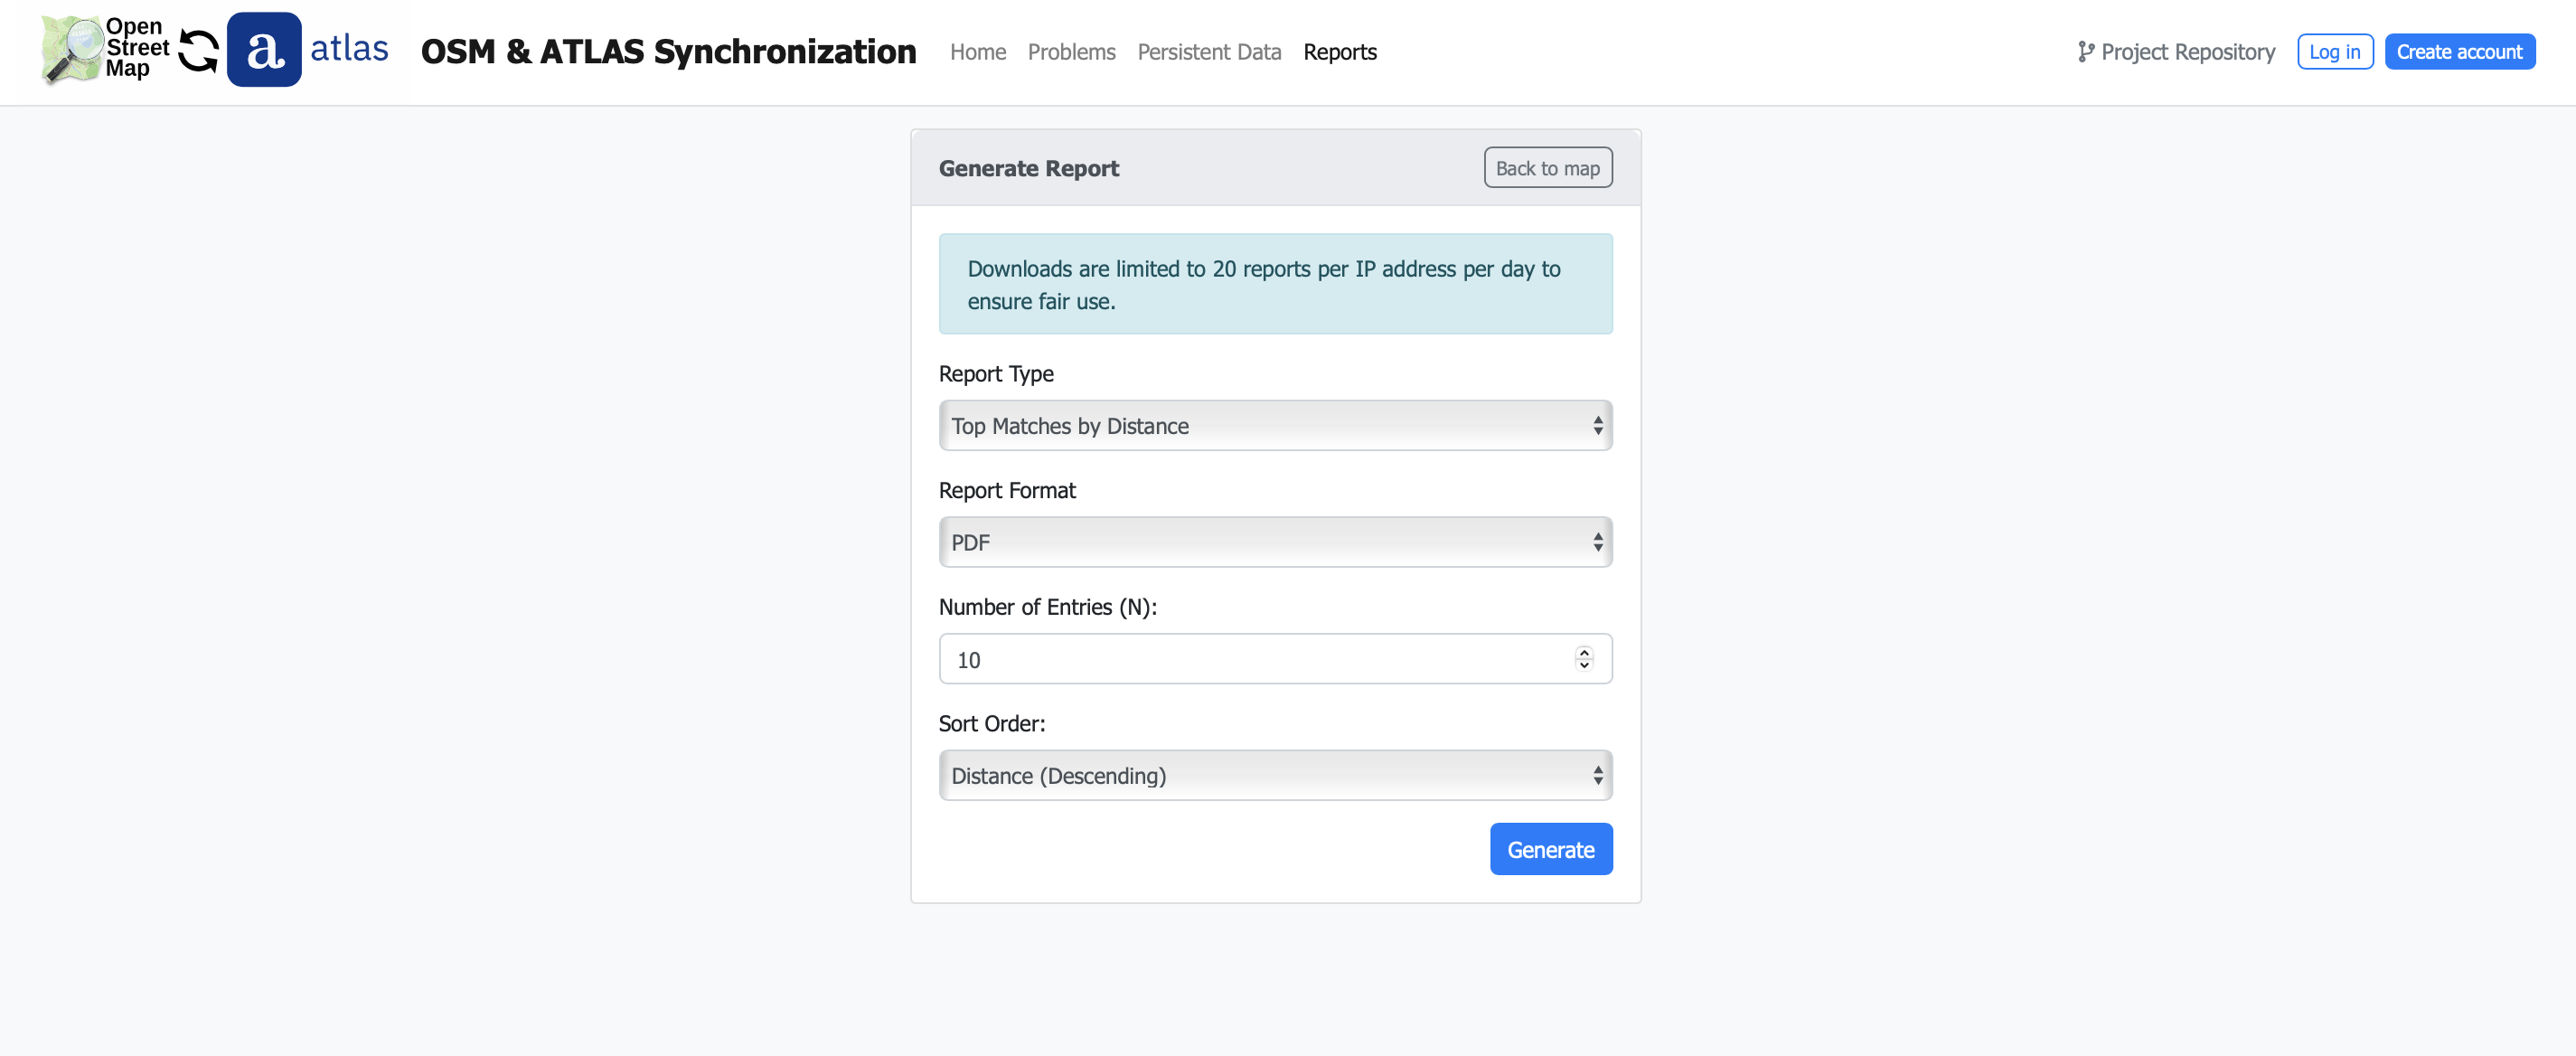
\includegraphics[width=0.9\textwidth]{../figures/chap9/download reports page.png}
  \caption[Page Rapports]{Page Rapports — génération (PDF/CSV) et limite quotidienne}
  \label{fig:frontend-report}
\end{figure}

\section{Liaison avec le backend (rappel Chap. 8)}

La cohérence et la réactivité de l'interface reposent sur:
\begin{itemize}
  \item \texttt{/api/data} — charge utile \textbf{minimale} pour la navigation (coordonnées, types, distance, identifiants).
  \item \texttt{/api/stop\_popup} — \textbf{détails} à la demande pour les info-bulles.
  \item \texttt{/api/top\_matches}, \texttt{/api/global\_stats} — \textbf{synthèses} parallèles non bloquantes.
  \item \texttt{/api/manual\_match}, \texttt{/api/save\_solution}, \texttt{/api/make\_solution\_persistent}, \texttt{/api/save\_note} — actions \textbf{créatrices} assorties d'une option de persistance.
\end{itemize}

Ces endpoints, leurs limites de débit et la sérialisation \texttt{format\_stop\_data()} sont détaillés au Chapitre~8.

\section*{Conclusion}

Le frontend associe une carte \textbf{fluide} (anti-rebond, annulation, seuils de zoom) à des \textbf{filtres expressifs} et à des info-bulles \textbf{paresseuses} pour conserver des charges utiles petites. L'outil Problèmes structure le travail de gestion des données et  persistance des données rendant les corrections \textbf{durables} entre imports. La génération de rapports complète l'ensemble en offrant des exports soignés.
